\documentclass[
	% -- opções da classe memoir --
	12pt,				% tamanho da fonte
	openright,			% capítulos começam em pág ímpar (insere página vazia caso preciso)
	oneside,			% para impressão em recto e verso. Oposto a oneside
	a4paper,			% tamanho do papel. 
	% -- opções da classe abntex2 --
	%chapter=TITLE,		% títulos de capítulos convertidos em letras maiúsculas
	%section=TITLE,		% títulos de seções convertidos em letras maiúsculas
	%subsection=TITLE,	% títulos de subseções convertidos em letras maiúsculas
	%subsubsection=TITLE,% títulos de subsubseções convertidos em letras maiúsculas
	% -- opções do pacote babel --
	english,			% idioma adicional para hifenização
	french,				% idioma adicional para hifenização
	spanish,			% idioma adicional para hifenização
	brazil				% o último idioma é o principal do documento
	]{abntex2}

% ---
% Pacotes básicos 
% ---
\usepackage{lmodern}			% Usa a fonte Latin Modern			
\usepackage[T1]{fontenc}		% Selecao de codigos de fonte.
\usepackage[utf8]{inputenc}		% Codificacao do documento (conversão automática dos acentos)
\usepackage{lastpage}			% Usado pela Ficha catalográfica
\usepackage{indentfirst}		% Indenta o primeiro parágrafo de cada seção.
\usepackage{color}		% Controle das cores
\usepackage{graphicx}			% Inclusão de gráficos
\usepackage{microtype} 			% para melhorias de justificação
\usepackage{diagbox} %tabelas com barras
% ---
		
% ---
% Pacotes adicionais, usados apenas no âmbito do Modelo Canônico do abnteX2
% ---
\usepackage{lipsum}				% para geração de dummy text
% ---

% ---
% Pacotes de citações
% ---
\usepackage[brazilian,hyperpageref]{backref}	 % Paginas com as citações na bibl
\usepackage[alf]{abntex2cite}	% Citações padrão ABNT

% --- 
% Pacotes matemáticos
% ---
\usepackage{amsthm}
% --- 
% CONFIGURAÇÕES DE PACOTES
% --- 
\newtheorem{definition}{Definição}
\newtheorem{teorema}{Teorema}
\newtheorem{corolario}{Corolário}
\graphicspath{{figuras/}}
% ---
% Configurações do pacote backref
% Usado sem a opção hyperpageref de backref
\renewcommand{\backrefpagesname}{Citado na(s) página(s):~}
% Texto padrão antes do número das páginas
\renewcommand{\backref}{}
% Define os textos da citação
\renewcommand*{\backrefalt}[4]{
	\ifcase #1 %
		Nenhuma citação no texto.%
	\or
		Citado na página #2.%
	\else
		Citado #1 vezes nas páginas #2.%
	\fi}%
% ---

% ---
% Informações de dados para CAPA e FOLHA DE ROSTO
% ---
\titulo{Análise de complexidade parametrizada em problemas de coloração para Grafos(r,l)}
\autor{Matheus Souza D'Andrea Alves}
\local{Niterói\\Rio de Janeiro\\Brasil}
\data{2017}
\orientador{Uéverton dos Santos Souza}
\coorientador{Raquel de Souza Fransisco Bravo}
\instituicao{%
  Universidade Federal Fluminense -- UFF
  \par
  Instituto de Computação}
\tipotrabalho{Trabalho de conclusão de curso}
% O preambulo deve conter o tipo do trabalho, o objetivo, 
% o nome da instituição e a área de concentração 
\preambulo{Trabalho de conclusão de curso submetido para obtenção do título de bacharel em Ciência da Computação concedido pelo Instituto de Computação da Universidade Federal Fluminense}
% ---


% ---
% Configurações de aparência do PDF final

% alterando o aspecto da cor azul
\definecolor{blue}{RGB}{41,5,195}

% informações do PDF
\makeatletter
\hypersetup{
     	%pagebackref=true,
		pdftitle={\@title}, 
		pdfauthor={\@author},
    	pdfsubject={\imprimirpreambulo},
	    pdfcreator={LaTeX with abnTeX2},
		pdfkeywords={grafos}{graphs}{complexity}{partitioning}{trabalho acadêmico}, 
		colorlinks=true,       		% false: boxed links; true: colored links
    	linkcolor=blue,          	% color of internal links
    	citecolor=blue,        		% color of links to bibliography
    	filecolor=magenta,      		% color of file links
		urlcolor=blue,
		bookmarksdepth=4
}
\makeatother
% --- 

% --- 
% Espaçamentos entre linhas e parágrafos 
% --- 

% O tamanho do parágrafo é dado por:
\setlength{\parindent}{1.3cm}

% Controle do espaçamento entre um parágrafo e outro:
\setlength{\parskip}{0.2cm}  % tente também \onelineskip

% ---
% compila o indice
% ---
\makeindex
% ---

% ----
% Início do documento
% ----
\begin{document}

% Seleciona o idioma do documento (conforme pacotes do babel)
%\selectlanguage{english}
\selectlanguage{brazil}

% Retira espaço extra obsoleto entre as frases.
\frenchspacing 

% ----------------------------------------------------------
% ELEMENTOS PRÉ-TEXTUAIS
% ----------------------------------------------------------
% \pretextual

% ---
% Capa
% ---
\imprimircapa
% ---

% ---
% Folha de rosto
% (o * indica que haverá a ficha bibliográfica)
% ---
\imprimirfolhaderosto*
% ---

% ---
% Inserir a ficha bibliografica
% ---

% Isto é um exemplo de Ficha Catalográfica, ou ``Dados internacionais de
% catalogação-na-publicação''. Você pode utilizar este modelo como referência. 
% Porém, provavelmente a biblioteca da sua universidade lhe fornecerá um PDF
% com a ficha catalográfica definitiva após a defesa do trabalho. Quando estiver
% com o documento, salve-o como PDF no diretório do seu projeto e substitua todo
% o conteúdo de implementação deste arquivo pelo comando abaixo:
%
% \begin{fichacatalografica}
%     \includepdf{fig_ficha_catalografica.pdf}
% \end{fichacatalografica}

\begin{fichacatalografica}
	\sffamily
	\vspace*{\fill}					% Posição vertical
	\begin{center}					% Minipage Centralizado
	\fbox{\begin{minipage}[c][8cm]{13.5cm}		% Largura
	\small
	\imprimirautor
	%Sobrenome, Nome do autor
	
	\hspace{0.5cm} \imprimirtitulo  / \imprimirautor. --
	\imprimirlocal, \imprimirdata-
	
	\hspace{0.5cm} \pageref{LastPage} p. : il. (algumas color.) ; 30 cm.\\
	
	\hspace{0.5cm} \imprimirorientadorRotulo~\imprimirorientador\\
	
	\hspace{0.5cm}
	\parbox[t]{\textwidth}{\imprimirtipotrabalho~--~\imprimirinstituicao,
	\imprimirdata.}\\
	
	\hspace{0.5cm}
		1. Palavra-chave1.
		2. Palavra-chave2.
		2. Palavra-chave3.
		I. Orientador.
		II. Universidade xxx.
		III. Faculdade de xxx.
		IV. Título 			
	\end{minipage}}
	\end{center}
\end{fichacatalografica}
% ---

% ---
% Inserir errata
% ---
% \begin{errata}
% Elemento opcional da \citeonline[4.2.1.2]{NBR14724:2011}. Exemplo:
%
% \vspace{\onelineskip}
%
% FERRIGNO, C. R. A. \textbf{Tratamento de neoplasias ósseas apendiculares com
% reimplantação de enxerto ósseo autólogo autoclavado associado ao plasma
% rico em plaquetas}: estudo crítico na cirurgia de preservação de membro em
% cães. 2011. 128 f. Tese (Livre-Docência) - Faculdade de Medicina Veterinária e
% Zootecnia, Universidade de São Paulo, São Paulo, 2011.
%
% \begin{table}[htb]
% \center
% \footnotesize
% \begin{tabular}{|p{1.4cm}|p{1cm}|p{3cm}|p{3cm}|}
%   \hline
%    \textbf{Folha} & \textbf{Linha}  & \textbf{Onde se lê}  & \textbf{Leia-se}  \\
%     \hline
%     1 & 10 & auto-conclavo & autoconclavo\\
%    \hline
% \end{tabular}
% \end{table}
%
% \end{errata}
% ---

% ---
% Inserir folha de aprovação
% ---

% Isto é um exemplo de Folha de aprovação, elemento obrigatório da NBR
% 14724/2011 (seção 4.2.1.3). Você pode utilizar este modelo até a aprovação
% do trabalho. Após isso, substitua todo o conteúdo deste arquivo por uma
% imagem da página assinada pela banca com o comando abaixo:
%
% \includepdf{folhadeaprovacao_final.pdf}
%
\begin{folhadeaprovacao}

  \begin{center}
    {\ABNTEXchapterfont\large\imprimirautor}

    \vspace*{\fill}\vspace*{\fill}
    \begin{center}
      \ABNTEXchapterfont\bfseries\Large\imprimirtitulo
    \end{center}
    \vspace*{\fill}
    
    \hspace{.45\textwidth}
    \begin{minipage}{.5\textwidth}
        \imprimirpreambulo
    \end{minipage}%
    \vspace*{\fill}
   \end{center}
        
   Trabalho aprovado. \imprimirlocal, 24 de novembro de 2012:

   \assinatura{\textbf{\imprimirorientador} \\ Orientador} 
   \assinatura{\textbf{Professor} \\ Convidado 1}
   \assinatura{\textbf{Professor} \\ Convidado 2}
   %\assinatura{\textbf{Professor} \\ Convidado 3}
   %\assinatura{\textbf{Professor} \\ Convidado 4}
      
   \begin{center}
    \vspace*{0.5cm}
    {\large\imprimirlocal}
    \par
    {\large\imprimirdata}
    \vspace*{1cm}
  \end{center}
  
\end{folhadeaprovacao}
% ---

% ---
% Dedicatória
% ---
\begin{dedicatoria}
   \vspace*{\fill}
   \centering
   \noindent
   \textit{ Dedicatória} \vspace*{\fill}
\end{dedicatoria}
% ---

% ---
% Agradecimentos
% ---
\begin{agradecimentos}


\end{agradecimentos}
% ---

% ---
% Epígrafe
% ---
\begin{epigrafe}
    \vspace*{\fill}
	\begin{flushright}
		\textit{"Ignorance more frequently begets confidence than does knowledge:\\
		It is those who know little, and not those who know much,\\ who so positively assert that this or that problem\\ will never be solved by science.\\
		Charles Darwin (The Descent of Man - pg 3)}
	\end{flushright}
\end{epigrafe}
% ---

% ---
% RESUMOS
% ---

% resumo em português
\setlength{\absparsep}{18pt} % ajusta o espaçamento dos parágrafos do resumo
\begin{resumo}
 O trabalho apresentado a seguir tem como proposta desvendar e catalogar a complexidade
 de problemas clássicos para a classe de Grafos(2,1), aprofundar em alguns deles quanto
 a complexidade parametrizada e extender as descobertas para Grafos(r,l).\\
 Para tanto utilizaremos do conhecimento prévio de complexidade para Grafos \textit{Split}
 e Grafos Bipartidos.
 
 \vspace{\onelineskip}
 
 \textbf{Palavras-chave}: Complexidade parametrizada. Grafos(r,l). Partição de grafos.
\end{resumo}

% resumo em inglês
\begin{resumo}[Abstract]
 \begin{otherlanguage*}{english}
   The work presented in this paper has the purpose of find and catalog the complexity
   of classical problems for the Graph(2,1) graph class, probe some of those about their 
   parametrized complexity and extend the findings to the Graph(r,l) graph class\\
   In way of doing so we will use de previous knowledge about thee complexity of problems for the
   Split and Bipartide graph classes

   \vspace{\onelineskip}
 
   \noindent 
   \textbf{Keywords}: latex. abntex. text editoration.
 \end{otherlanguage*}
\end{resumo}
% ---

% ---
% inserir lista de ilustrações
% ---
\pdfbookmark[0]{\listfigurename}{lof}
\listoffigures*
\cleardoublepage
% ---

% ---
% inserir lista de tabelas
% ---
\pdfbookmark[0]{\listtablename}{lot}
\listoftables*
\cleardoublepage
% ---

% ---
% inserir lista de abreviaturas e siglas
% ---
\begin{siglas}
  \item[\textit{P}] Complexidade de tempo Polinomial determinístico
  \item[\textit{NPc}] Complexidade de tempo Polinomial não determinístico completa
\end{siglas}
% % ---
%
% % ---
% % inserir lista de símbolos
% % ---
% \begin{simbolos}
%   \item[$ \Gamma $] Letra grega Gama
%   \item[$ \Lambda $] Lambda
%   \item[$ \zeta $] Letra grega minúscula zeta
%   \item[$ \in $] Pertence
% \end{simbolos}
% ---

% ---
% inserir o sumario
% ---
\pdfbookmark[0]{\contentsname}{toc}
\tableofcontents*
\cleardoublepage
% ---



% ----------------------------------------------------------
% ELEMENTOS TEXTUAIS
% ----------------------------------------------------------
\textual

% ----------------------------------------------------------
% Introdução (exemplo de capítulo sem numeração, mas presente no Sumário)
% ----------------------------------------------------------
\chapter*[Introdução]{Introdução}
\addcontentsline{toc}{chapter}{Introdução}
% ----------------------------------------------------------
%
% Este documento e seu código-fonte são exemplos de referência de uso da classe
% \textsf{abntex2} e do pacote \textsf{abntex2cite}. O documento 
% exemplifica a elaboração de trabalho acadêmico (tese, dissertação e outros do
% gênero) produzido conforme a ABNT NBR 14724:2011 \emph{Informação e documentação
% - Trabalhos acadêmicos - Apresentação}.
%
% A expressão ``Modelo Canônico'' é utilizada para indicar que \abnTeX\ não é
% modelo específico de nenhuma universidade ou instituição, mas que implementa tão
% somente os requisitos das normas da ABNT. Uma lista completa das normas
% observadas pelo \abnTeX\ é apresentada em \citeonline{abntex2classe}.
%
% Sinta-se convidado a participar do projeto \abnTeX! Acesse o site do projeto em
% \url{http://www.abntex.net.br/}. Também fique livre para conhecer,
% estudar, alterar e redistribuir o trabalho do \abnTeX, desde que os arquivos
% modificados tenham seus nomes alterados e que os créditos sejam dados aos
% autores originais, nos termos da ``The \LaTeX\ Project Public
% License''\footnote{\url{http://www.latex-project.org/lppl.txt}}.
%
% Encorajamos que sejam realizadas customizações específicas deste exemplo para
% universidades e outras instituições --- como capas, folha de aprovação, etc.
% Porém, recomendamos que ao invés de se alterar diretamente os arquivos do
% \abnTeX, distribua-se arquivos com as respectivas customizações.
% Isso permite que futuras versões do \abnTeX~não se tornem automaticamente
% incompatíveis com as customizações promovidas. Consulte
% \citeonline{abntex2-wiki-como-customizar} par mais informações.
%
% Este documento deve ser utilizado como complemento dos manuais do \abnTeX\ 
% \cite{abntex2classe,abntex2cite,abntex2cite-alf} e da classe \textsf{memoir}
% \cite{memoir}. 
%
% Esperamos, sinceramente, que o \abnTeX\ aprimore a qualidade do trabalho que
% você produzirá, de modo que o principal esforço seja concentrado no principal:
% na contribuição científica.
%
% Equipe \abnTeX 
%
% Lauro César Araujo

% ----------------------------------------------------------
% PARTE
% ----------------------------------------------------------
\part{Preparação da pesquisa}
% ----------------------------------------------------------

% ---
% Capitulo com exemplos de comandos inseridos de arquivo externo 
% ---
\include{abntex2-modelo-include-comandos}
% ---

% ----------------------------------------------------------
% PARTE
% ----------------------------------------------------------
\part{Análise do problema de coloração para Grafos(r,l)}
% ----------------------------------------------------------

% ---
% Capitulo de revisão de literatura
% ---
\chapter{Evolução do problema de coloração considerando o crescimento de r e l}
% ---

% ---
\section{Definição}
% ---

O problema de coloração em grafos pode ser definido como:

\begin{definition}
  Coloração em Grafos\\
  Entrada: um Grafo $G$ e um inteiro $k$\\
  Questão: Cada vértice pertencente à $G$ pode ser colorido com uma entre $k$ cores
  de tal forma que dado quaisquer dois vértices adjacentes eles tenham cores distintas e $k$ seja o mínimo de cores possível? 
\end{definition}

\section{Complexidade de coloração em Grafos(r,l)}

%Discorrer e comentar sobre soluções já conhecida para coloração (r,l)
Sabemos que coloração é de solução conhecidamente polinomial para clique, independente, grafos split e para grafos bipartidos.

Iremos demonstrar abaixo a complexidade para casos de ordem superiores. 
\begin{itemize}
  \item Grafo(1,2):
    \begin{teorema}
      Se lista coloração de grafos split é NPc então coloração de Grafos(1,2) é NPc
    \end{teorema}
    \begin{proof}
      A prova do teorema baseia-se em mostrar que uma solução de lista coloração para grafos split implica em uma solução para o problema de coloração de um Grafo(1,2) H, portanto para provarmos é preciso mostrar que
      \begin{itemize}
        \item Se um grafo split G possui uma lista coloração própria então H é k-colorível para k=nº de cores nas listas (1)
        \item Se H é k-colorível então G possui uma lista coloração própria (2)
      \end{itemize}
      (1):\newline
      \begin{figure}[!ht]
        \centering
        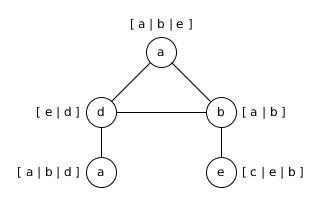
\includegraphics[width=0.5\textwidth]{split-1.png}
        \caption{Grafo G: Instância sim para o problema de lista coloração para split }
      \end{figure}
      Usaremos a seguinte construção:\newline
      Considere G um grafo split e que para cada vértice $v \in V(G)$ exista uma lista de cores $S_v$ referente a esse vértice, cada lista contém pelo menos uma cor do conjunto $C = \{c_1,c_2,c_3,...,c_k \}$, sendo G uma instância sim para o problema de lista coloração, criemos uma clique K onde cada vértice $k \in V(K)$ representa uma cor presente em $C$. Seja $H = G \cup K$ para todo vértice $v \in G$ e todo vértice $u_i \in K$ adicione uma aresta $(u_i,v)$ à H se e somente se v não possui a cor $c_i$ em sua lista coloração em G
      
      Podemos então generalizar da seguinte forma, dado um grafo split $G$ onde cada vértice de $G$ possui uma lista de possíveis cores então o grafo $H_G$ obtido pela construção anterior possui uma k-coloração.
      
      Note que a clique K possui exatamente k vértices, consequentemente para colorirmos K precisaremos de k cores, sem perda de generalidade assumimos que $u_1$ será colorido com $c_1$, $u_2$ com $c_2$ e assim por diante.
      
      Por construção uma aresta de $u_i$ só existe para $v_a$ em $H$ se e somente se, $v_a$ não possui $c_i$ em sua lista de cores, portanto a coloração atribuída à K não conflita com a com a lista coloração de G, e portanto para todo vértice perntecente a G podemos lhe atribuir a mesma cor que lhe foi atribuída no problema de lista coloração, obtendo uma coloração própria para H
      
      (2):\newline
      Suponha que o grafo $H_G$ possua uma K-coloração própria, onde k é o numero de cores nas listas de G
      
      Seja K a maior clique presente em $H_G$, por construção $H_G$ é colorível com k cores onde k é a cardinalidade de K, observe que a remoção de K não afeta a coloração de $H_G - K$
      
      Como $H_G$ é k-colorível e a clique K possui k vértices todas as cores de tal k-coloração estão presentes em K. Sem perda de generalidade podemos assumir que as cores $c_1,c_2,...,c_k$ estão atribuídas aos vértices $u_1,u_2,...,u_k$ pertencentes à K
      
      Por construção de $H_G$ todo par $(v,u_i)$ onde $v \in H_G - K$ e $u_i \in K$ é não adjacente se e somente se o vértice $v$ não possui $c_i$ em sua lista coloração no grafo $G$
      
      Logo a k-coloração atribuídas aos vértices em $H_G - K$ formam uma coloração para G onde todo vértice em $V(G)$ possui uma cor de sua lista. Portanto G é uma instância sim de lista coloração
    \end{proof}
    \begin{corolario}
    Seja G uma instância de lista coloração onde G é uma (r,l) partição e seja c o número de cores utilizadas em G, existe um grafo $H_G$ (k,l+1) particionável tal que G é uma instância sim de lista coloração, se e somente se $H_G$ é c-colorível
    \end{corolario}
    \begin{corolario}
    Se Lista coloração é NPc em Grafos(r,l) então Coloração é NPc em Grafos(r,l+1)
    \end{corolario}    
  \item Grafo(2,1)
  \item Grafo(3,0):\newline
      Tendo um Grafo G da classe (3,0) como entrada para o problema de coloração sabemos já que o grafo pode ser colorido com 3 cores, resta saber se 3 é o o numero mínimo de cores que pode ser usado, portanto devemos verificar se G é bipartido (colorível com 2 cores) ou um grafo sem arestas (colorível com 1 cor), como ambas verificações são polinomiais podemos afirmar que coloração de Grafo(3,0) é resolvível de forma polinomial.
  \item Grafo(4,0):
      \begin{teorema}
        Se 3-coloração de planar é NPc então coloração de Grafo(4,0) é NPc
      \end{teorema}
      \begin{proof}
        Sabemos que todo grafo planar é 4-colorível, e que alguns grafos(4,0) são planares, portanto sabemos que para qualquer Grafo G $\in$ subconjunto de planares de grafos(4,0), sua quantidade máxima de cores é 4, nos resta saber se 4 também é sua quantidade mínima, porém 3-coloração de planar é NPc logo descobrir a coloração mínima de G é NPc e consequentemente coloração de Grafos(4,0) é NPc
      \end{proof}
  \item Grafo(0,3)
      \begin{teorema}
        (?)Se lista coloração em Grafos(2,0) é NPc então coloração em Grafos(3,0) é NPc
      \end{teorema}
  \item Grafo(0,4)
      \begin{teorema}
      Se clique cover em planar é NPc então Coloração de Grafo(0,4) é NPc 
      \end{teorema}
      \begin{proof}
        Sabemos que o problema de coloração em qualquer grafo G é equivalente ao problema de clique cover no seu complemento $\overline G$, ou seja, para determinar a complexidade de coloração de Grafos(0,4) iremos determinar a complexidade de clique cover em Grafos(4,0), sabemos que um subconjunto de Grafos(4,0) são planares e que clique cover em planares é NPc, logo clique cover em Grafos(4,0) é NPc implicando que coloração em Grafos(0,4) seja NPc
      \end{proof}
\end{itemize}
portanto podemos obter a seguinte tabela:

\begin{table}[htb!]
  \center
  \begin{tabular}{l|*{6}c}
    \toprule
    \backslashbox{$k$}{$l$} & 0 & 1 & 2 & 3 & 4 & n\\
    \midrule
    0 & \textit{P} & \textit{P} & \textit{P} & ? & \textit{NPc} & \textit{NPc}\\
    1 & \textit{P} & \textit{P} & \textit{NPc} & \textit{NPc} & \textit{NPc} & \textit{NPc}\\
    2 & \textit{P} & \textit{NPc} & \textit{NPc} & \textit{NPc} & \textit{NPc} & \textit{NPc}\\
    3 & \textit{P} & \textit{NPc} & \textit{NPc} & \textit{NPc} & \textit{NPc} & \textit{NPc}\\
    4 & \textit{NPc} & \textit{NPc} & \textit{NPc} & \textit{NPc} & \textit{NPc} & \textit{NPc}\\
    n & \textit{NPc} & \textit{NPc} & \textit{NPc} & \textit{NPc} & \textit{NPc} & \textit{NPc}\\
    \bottomrule
  \end{tabular}%
  \caption{Complexidade do problema de coloração em Grafos(r,l)}
  \label{tab:tabela_coloraçãorl}%
\end{table}%

% ----------------------------------------------------------
% PARTE
% ----------------------------------------------------------
\part{Resultados}
% ----------------------------------------------------------

% ---
% primeiro capitulo de Resultados
% ---
\chapter{Lectus lobortis condimentum}
% ---

% ---
\section{Vestibulum ante ipsum primis in faucibus orci luctus et ultrices
posuere cubilia Curae}
% ---

\lipsum[21-22]

% ---
% segundo capitulo de Resultados
% ---
\chapter{Nam sed tellus sit amet lectus urna ullamcorper tristique interdum
elementum}
% ---

% ---
\section{Pellentesque sit amet pede ac sem eleifend consectetuer}
% ---

\lipsum[24]

% ----------------------------------------------------------
% Finaliza a parte no bookmark do PDF
% para que se inicie o bookmark na raiz
% e adiciona espaço de parte no Sumário
% ----------------------------------------------------------
\phantompart

% ---
% Conclusão
% ---
\chapter{Conclusão}
% ---

\lipsum[31-33]

% ----------------------------------------------------------
% ELEMENTOS PÓS-TEXTUAIS
% ----------------------------------------------------------
\postextual
% ----------------------------------------------------------

% ----------------------------------------------------------
% Referências bibliográficas
% ----------------------------------------------------------
\bibliography{modelo-referencias}

% ----------------------------------------------------------
% Glossário
% ----------------------------------------------------------
%
% Consulte o manual da classe abntex2 para orientações sobre o glossário.
%
%\glossary

% ----------------------------------------------------------
% Apêndices
% ----------------------------------------------------------

% ---
% Inicia os apêndices
% ---
\begin{apendicesenv}

% Imprime uma página indicando o início dos apêndices
\partapendices

% ----------------------------------------------------------
\chapter{Quisque libero justo}
% ----------------------------------------------------------

\lipsum[50]

% ----------------------------------------------------------
\chapter{Nullam elementum urna vel imperdiet sodales elit ipsum pharetra ligula
ac pretium ante justo a nulla curabitur tristique arcu eu metus}
% ----------------------------------------------------------
\lipsum[55-57]

\end{apendicesenv}
% ---


% ----------------------------------------------------------
% Anexos
% ----------------------------------------------------------

% ---
% Inicia os anexos
% ---
\begin{anexosenv}

% Imprime uma página indicando o início dos anexos
\partanexos

% ---
\chapter{Morbi ultrices rutrum lorem.}
% ---
\lipsum[30]

% ---
\chapter{Cras non urna sed feugiat cum sociis natoque penatibus et magnis dis
parturient montes nascetur ridiculus mus}
% ---

\lipsum[31]

% ---
\chapter{Fusce facilisis lacinia dui}
% ---

\lipsum[32]

\end{anexosenv}

%---------------------------------------------------------------------
% INDICE REMISSIVO
%---------------------------------------------------------------------
\phantompart
\printindex
%---------------------------------------------------------------------

\end{document}
